\documentclass{article}
\usepackage[utf8]{inputenc}
\usepackage[spanish]{babel}
\usepackage{listings}
\usepackage{graphicx}
\graphicspath{ {images/} }
\usepackage{cite}

\begin{document}

\begin{titlepage}
    \begin{center}
        \vspace*{4cm}
            
        \Huge
        \textbf{Manual de intrucciones}
            
        \vspace{0.5cm}
        \LARGE
        Encendido de matriz 8x8\\ Informa2 S.A.S
            
        \vspace{1.5cm}
            
  
            
        \vfill
            
        \vspace{0.8cm}
            
        \Large
        Despartamento de Ingeniería Electrónica y Telecomunicaciones\\
        Universidad de Antioquia\\
        Medellín\\
        Abril de 2021
            
    \end{center}
\end{titlepage}

\tableofcontents
\newpage

 Mediante esta guía se pretende que el usuario de la aplicación sepa el funcionamiento de esta.Se le indicará que comandos debe ejecutar por el Monitor en serie para obtener diferetes resultados\\

\textbf{Menú}: El usuario puede observar un menú principal 
donde encontrará las sigueinte 4 opciones:

    \begin{figure}[h]
    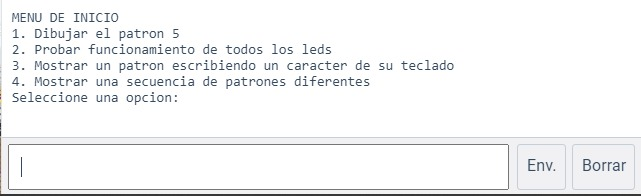
\includegraphics[width=13cm]{menu.jpeg}
    \centering
    \caption{Menú principal}
    \label{menu}
    \end{figure}

\section{Dibujar el patrón "5"}\label{op1}
La escogencia de la opción 1 llevará al usuario a observar un patrón determinado de la matriz,más especificamente el patrón 5 (ver figura 1).Cabe aclarar que el usuario para elegir esta opción debe pulsar la tecla 1 de su teclado.

    \begin{figure}[h]
    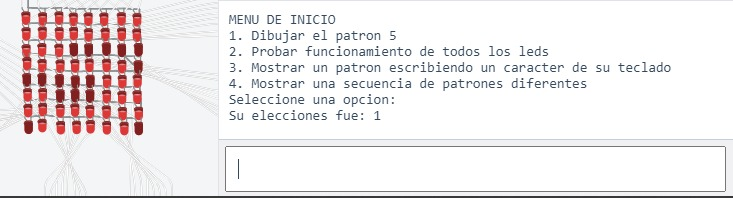
\includegraphics[width=13cm]{5.jpeg}
    \centering
    \caption{Patrón de prueba número "5"}
    \label{5}
    \end{figure}
    
\section{Probar funcionamiento de todos los LEDs}\label{op2}
Al escoger esta opción, el programa le permitirá al usuario verificar que todos los LEDs esten en óptimo funcionamiento,es decir que todos los LEDs pertencientes a la matriz enciendan.

    \begin{figure}[h]
    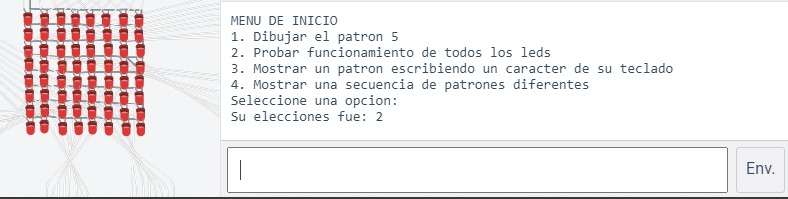
\includegraphics[width=13cm]{full.jpeg}
    \centering
    \caption{Patrón de prueba todos LEDs encendidos}
    \label{full}
    \end{figure}

\section{Mostrar un patrón escribiendo una carácter de su tecado}\label{op3}
En esta opción el programa solicitará al usuario ingresar un carácter,únicamente el usuario podrá ingresar una letra entre la A y Z o un número entre el cero (0) y el nueve (9). Dentro de las letras el usuario puede ingresar minúsculas o mayúsculas.Si el usuario ingresa un carácter diferente a los mencionados, se motrará un patrón que refleja un signo de pregunta, indicando así que el sistema no reconoce el carácter ingresado.

    \begin{figure}[h]
    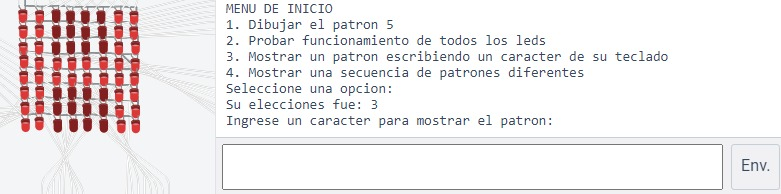
\includegraphics[width=13cm]{patron.jpeg}
    \centering
    \caption{Carácter digitado por el usuario}
    \label{patron}
    \end{figure}
    
\section{Mostrar una secuencia de patrones diferentes}\label{op4}
Cuando el usuario escoge esta opción en primer lugar el programa solicitará el tiempo de duración entre patrón y el siguiente, luego entonces se le pedirá ingresar una palabra compuesta por varios carácteres, cabe aclarar que si el usuario ingresa un carácter diferente a una letra o un número dentro de la secuencia de patrones se desplegará un signo de interrogación en el carácter que el programa no reconozca.

    \begin{figure}[h]
    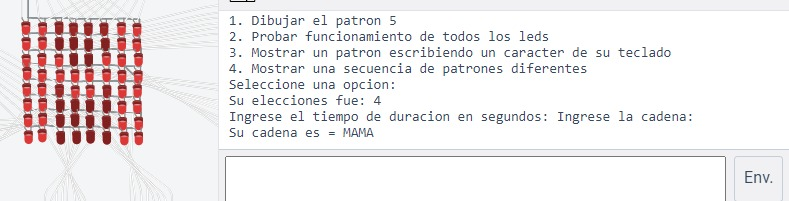
\includegraphics[width=13cm]{Ma.jpeg}
    \centering
    \caption{Letra M en la secuencia "MAMA" }
    \label{ma}
    \end{figure}

    \begin{figure}[h]
    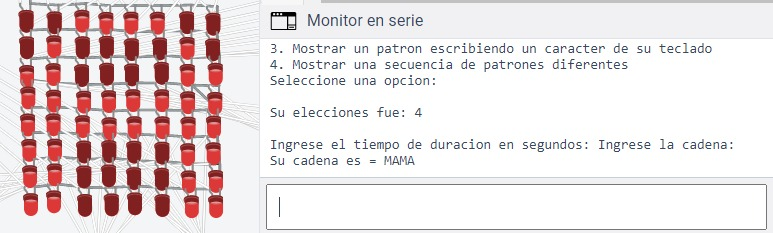
\includegraphics[width=13cm]{A.jpeg}
    \centering
    \caption{Letra A en la secuencia "MAMA" }
    \label{a}
    \end{figure}
    
\bibliographystyle{IEEEtran}

\end{document}
